% CC-BY-4.0; Copyright (c) 2026 Jonathan Yantis. Generated by tools/verify_power.py
\documentclass[border=5pt]{standalone}
\usepackage{pgfplots}
\pgfplotsset{compat=1.18}
\definecolor{studyblue}{RGB}{39,83,109}
\definecolor{studyorange}{RGB}{180,94,32}
\begin{document}
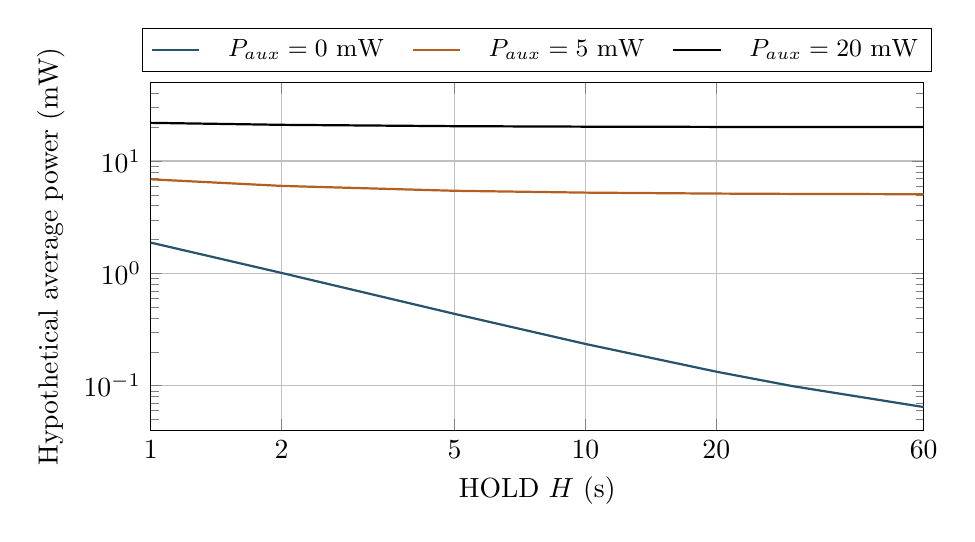
\begin{tikzpicture}\begin{axis}[width=.94\linewidth,height=6cm,xmode=log,ymode=log,xmin=1,xmax=60,xtick={1,2,5,10,20,60},xticklabels={1,2,5,10,20,60},ymin=.04,ymax=50,xlabel={HOLD $H$ (s)},ylabel={Hypothetical average power (mW)},legend style={column sep=.8em,font=\small,at={(.5,1.03)},anchor=south,legend columns=3},grid=major]
\addplot[studyblue,thick] coordinates {(1,1.879813333) (2,1.009312941) (5,0.4360565854) (10,0.2355348148) (20,0.1334057143) (30,0.09908016598) (60,0.06461189189)};\addlegendentry{$P_{aux}=0$ mW}
\addplot[studyorange,thick] coordinates {(1,6.879813333) (2,6.009312941) (5,5.436056585) (10,5.235534815) (20,5.133405714) (30,5.099080166) (60,5.064611892)};\addlegendentry{$P_{aux}=5$ mW}
\addplot[black,thick] coordinates {(1,21.87981333) (2,21.00931294) (5,20.43605659) (10,20.23553481) (20,20.13340571) (30,20.09908017) (60,20.06461189)};\addlegendentry{$P_{aux}=20$ mW}
\end{axis}\end{tikzpicture}
\end{document}
